\section{Uygulama I}
Bu bölümde beş farklı kısımdan oluşan bir konsol kirişin boyut optimizasyonu gösterilecektir.

\sidenote{
    
\qrcode[height=1in]{https://github.com/btayfur/structural-optimization/blob/main/Code/Examples/Exmp6/}}

\subsection{Problem Tanımı}
Bu uygulamada, 5 eşit parçadan oluşan 3 metre uzunluğundaki bir konsol kirişin ağırlığını minimize etmeyi amaçlayan bir optimizasyon problemi ele alınacaktır. Problemin detayları şu şekildedir:

\begin{itemize}
    \item 3 metre uzunluğunda, 5 eşit parçaya bölünmüş bir konsol kiriş
    \item Her bir parçanın içi boş dairesel kesiti vardır ve iki tasarım parametresi bulunur:
    \begin{itemize}
        \item $r_{dış}$: Dış yarıçap
        \item $r_{iç}$: İç yarıçap
    \end{itemize}
    \item Malzeme: S270 çeliği (E = 210 GPa, $\sigma_y$ = 270 MPa)
    \item Kirişin serbest ucuna dik olarak F = 500 kN'luk bir kuvvet uygulanmaktadır
    \item Amaç: Kirişin ağırlığını minimize etmek
\end{itemize}

\subsubsection{Kısıtlamalar}
\begin{enumerate}
    \item Kirişin serbest ucunda maksimum 2 cm'lik bir deplasman izin verilmektedir
    \item Her bir parça için dış yarıçap, iç yarıçaptan büyük olmalıdır
    \item Bir önceki parçanın iç yarıçapı, bir sonraki parçanın dış yarıçapından küçük olmalıdır (kaynak yapılabilirlik koşulu)
    \item S270 çeliğinin akma gerilmesi (270 MPa) aşılmamalıdır
\end{enumerate}

\subsection{Yapısal Analiz}
Konsol kirişin deplasman ve gerilme analizi için sonlu elemanlar yöntemi kullanılmıştır:

\begin{itemize}
    \item Her kiriş parçası bir Euler-Bernoulli kiriş elemanı olarak modellenmiştir
    \item Her düğüm noktasında 2 serbestlik derecesi vardır (deplasman ve dönme)
    \item Deplasmanları hesaplamak için global rijitlik matrisi oluşturulmuştur
    \item Gerilmeler, eğilme momenti ve kesit özellikleri kullanılarak hesaplanmıştır
\end{itemize}

\subsubsection{Rijitlik Matrisi Oluşturma}
Kiriş elemanı için rijitlik matrisi şu şekilde oluşturulur:

\begin{equation}
k_e = \begin{bmatrix}
\frac{12EI}{l^3} & \frac{6EI}{l^2} & -\frac{12EI}{l^3} & \frac{6EI}{l^2} \\
\frac{6EI}{l^2} & \frac{4EI}{l} & -\frac{6EI}{l^2} & \frac{2EI}{l} \\
-\frac{12EI}{l^3} & -\frac{6EI}{l^2} & \frac{12EI}{l^3} & -\frac{6EI}{l^2} \\
\frac{6EI}{l^2} & \frac{2EI}{l} & -\frac{6EI}{l^2} & \frac{4EI}{l}
\end{bmatrix}
\end{equation}

Burada:
\begin{itemize}
    \item $E$: Young modülü
    \item $I$: Atalet momenti
    \item $l$: Eleman uzunluğu
\end{itemize}

İçi boş dairesel kesit için atalet momenti:
\begin{equation}
I = \frac{\pi}{4}(r_{dış}^4 - r_{iç}^4)
\end{equation}

\subsubsection{Sınır Koşulları ve Çözüm}
Konsol kirişin sol ucu sabitlenmiştir, bu nedenle ilk düğüm noktasındaki serbestlik dereceleri sıfırdır. Sağ uca uygulanan kuvvet, global kuvvet vektörüne eklenir. Deplasman vektörü, indirgenmiş rijitlik matrisi ve kuvvet vektörü kullanılarak çözülür:

\begin{equation}
\mathbf{K_{indirgenmiş}} \cdot \mathbf{u} = \mathbf{F}
\end{equation}

\subsection{Optimizasyon Yaklaşımı}
Optimizasyon için Tavlama Benzetimi (Simulated Annealing) algoritması kullanılmıştır:

\begin{itemize}
    \item Yerel optimumlardan kaçınmak için rastgele arama stratejisi
    \item Çözüm uzayının etkili bir şekilde keşfi için adaptif adım boyutu
    \item Daha iyi çözümler bulmak için süreç sıcaklığının yavaş soğutulması
    \item Fiziksel olarak uygulanabilir çözümleri sağlamak için kısıtlamaların etkin kontrolü
\end{itemize}

\subsubsection{Amaç Fonksiyonu}
Amaç fonksiyonu, kirişin toplam ağırlığıdır:

\begin{equation}
W = \rho \sum_{i=1}^{5} A_i \cdot l_i
\end{equation}

Burada:
\begin{itemize}
    \item $\rho$: Malzeme yoğunluğu
    \item $A_i$: Her bir parçanın kesit alanı ($A_i = \pi(r_{dış,i}^2 - r_{iç,i}^2)$)
    \item $l_i$: Her bir parçanın uzunluğu
\end{itemize}

\subsubsection{Kısıtlama Fonksiyonları}
Optimizasyon sürecinde dört kısıtlama fonksiyonu kullanılmıştır:

\begin{enumerate}
    \item Deplasman kısıtlaması: $u_{max} \leq 0.02$ m
    \item Yarıçap kısıtlaması: $r_{dış,i} > r_{iç,i}$ (her parça için)
    \item Kaynak yapılabilirlik kısıtlaması: $r_{iç,i} < r_{dış,i+1}$ (bitişik parçalar için)
    \item Gerilme kısıtlaması: $\sigma_{max} \leq \sigma_{yield}$
\end{enumerate}

\subsection{Optimizasyon Sonuçları}
Optimizasyon, başlangıç tasarımına kıyasla daha hafif bir kiriş tasarımı ile sonuçlanmıştır:

\begin{itemize}
    \item Başlangıç tasarımının ağırlığı: $\sim$1924 kg
    \item Optimize edilmiş tasarımın ağırlığı: $\sim$939 kg (\%51 azalma)
\end{itemize}

\begin{figure}[H]
    \centering
    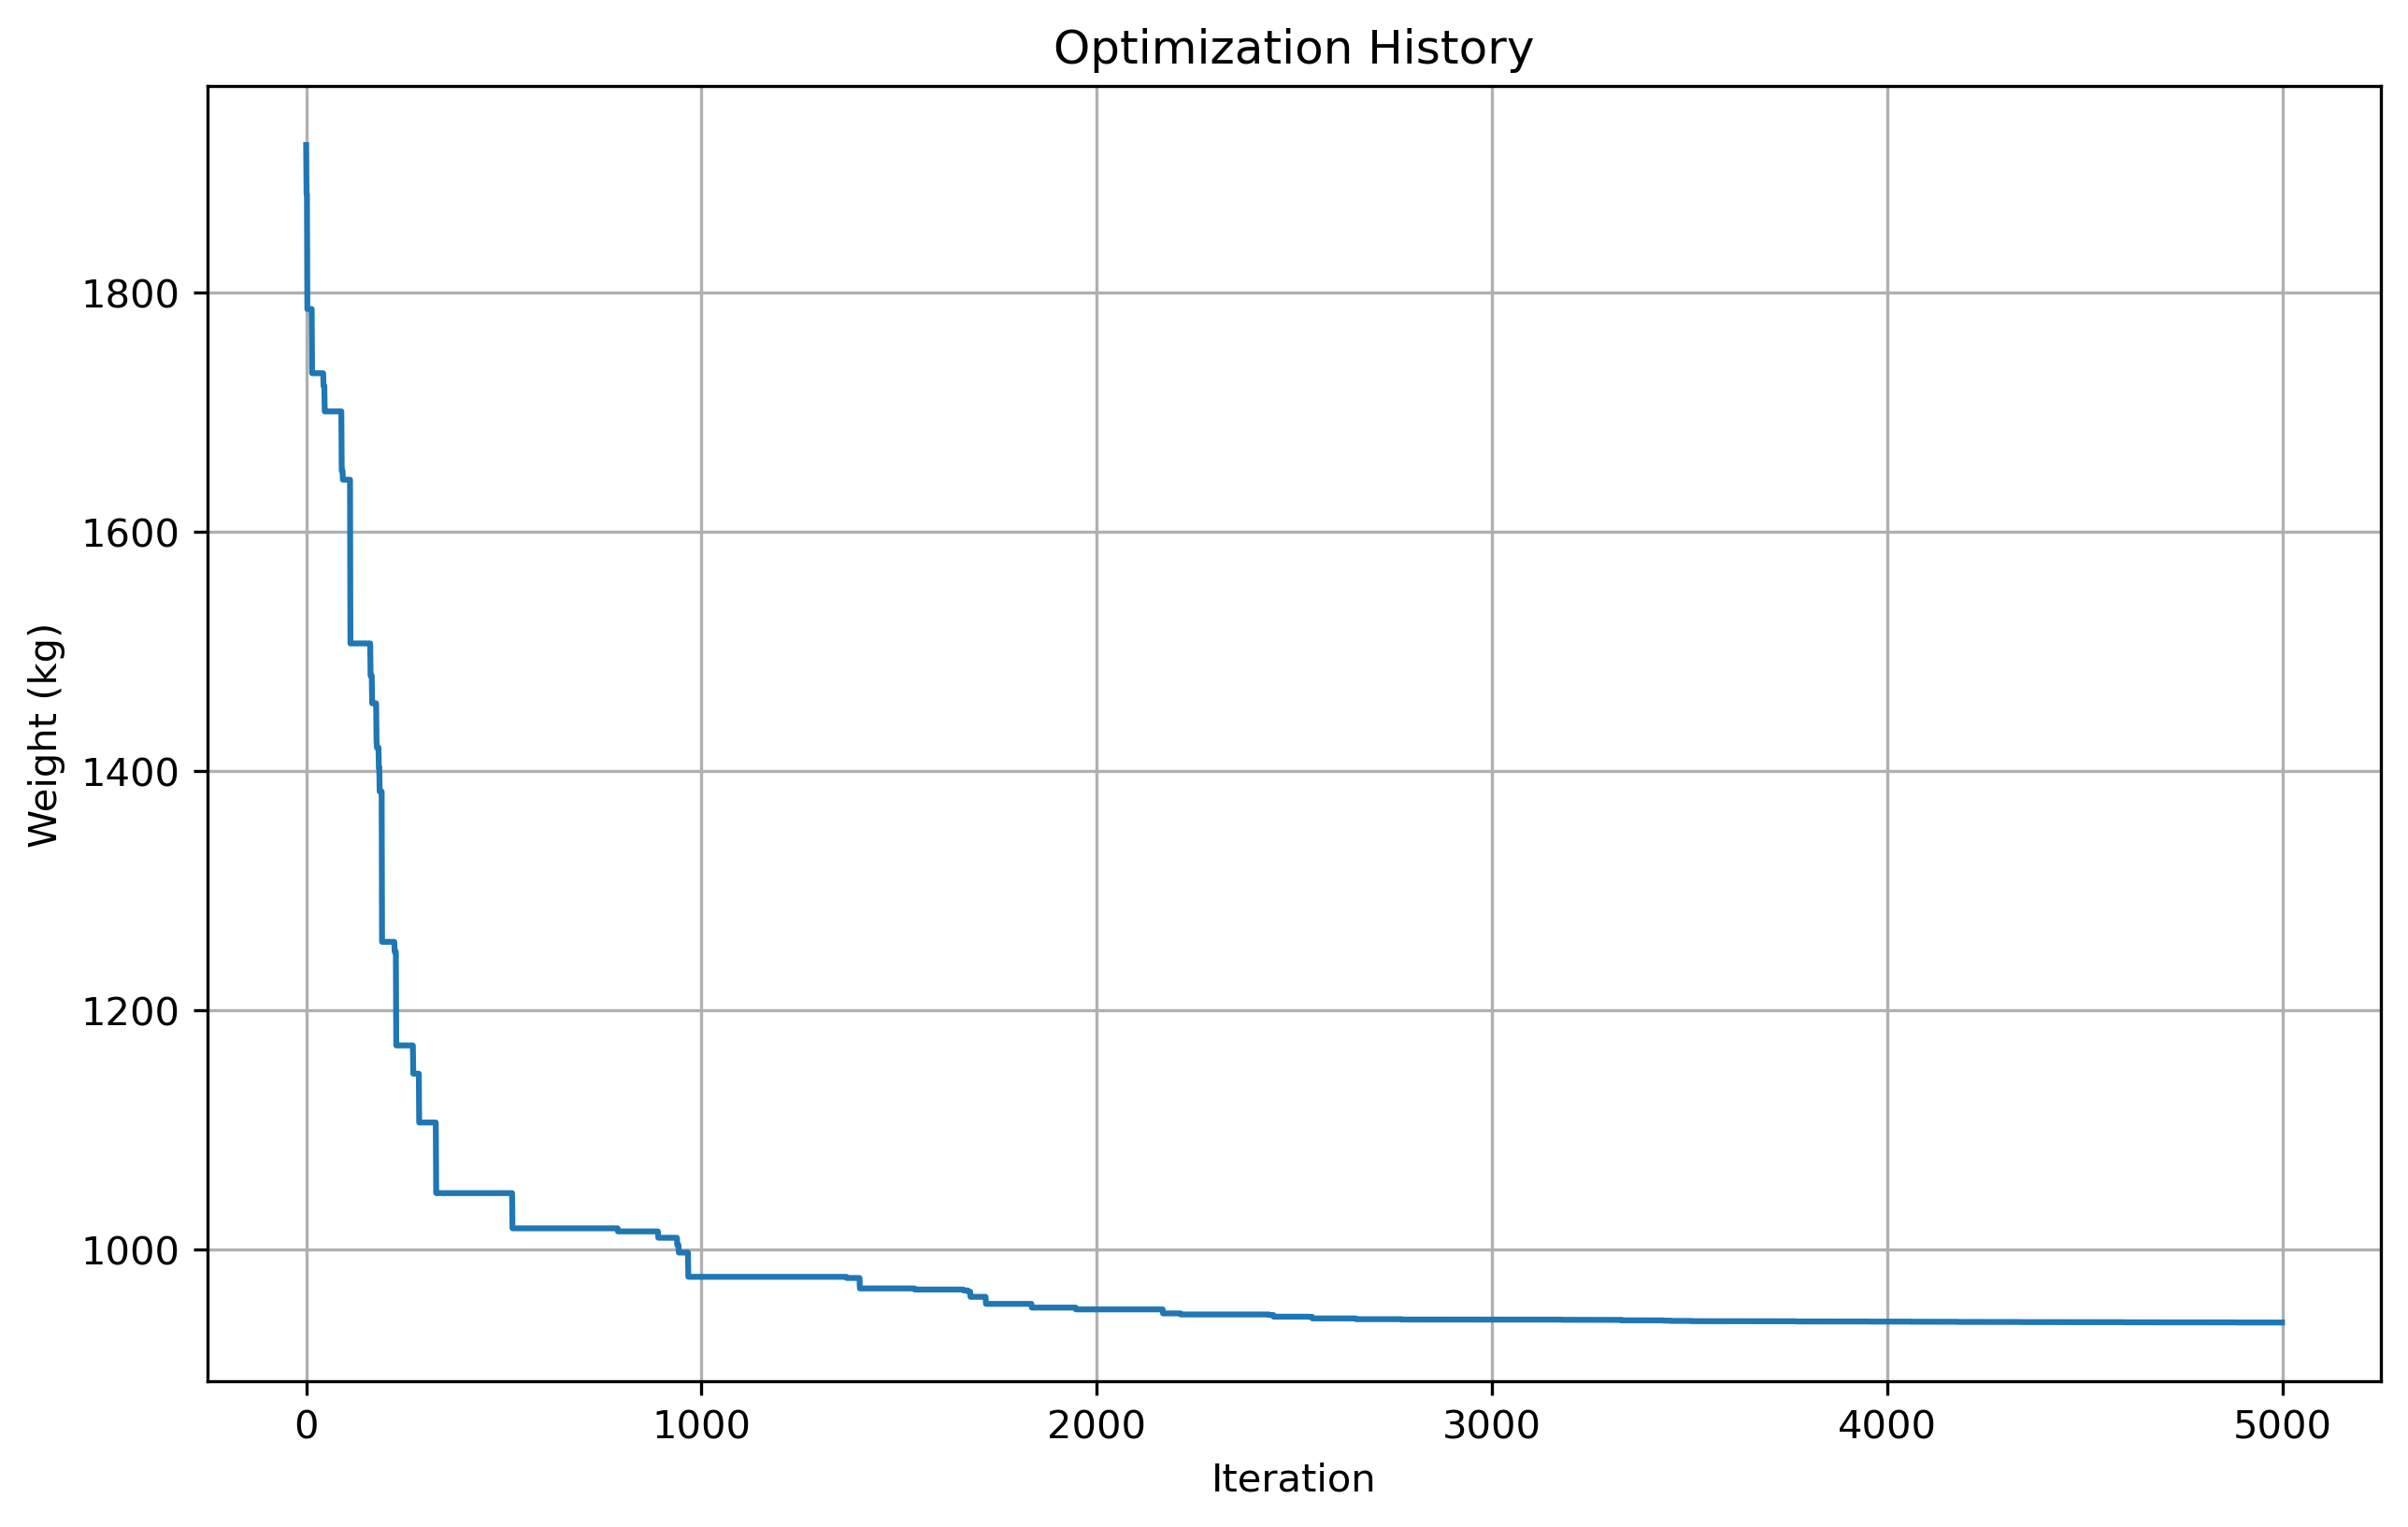
\includegraphics[width=1\textwidth]{weeks_new/imgs/optimization_history.png}
    \caption{Ağırlık İzleme Grafiği}
    \label{fig:optimization_history}
\end{figure}

\subsubsection{Optimize Edilmiş Yarıçaplar (cm)}
\begin{center}
\begin{tabular}{|c|c|c|}
\hline
Parça & Dış Yarıçap ($r_{dış}$) & İç Yarıçap ($r_{iç}$) \\
\hline
1 & 20.37 & 14.36 \\
2 & 20.05 & 15.81 \\
3 & 15.82 & 9.04 \\
4 & 16.00 & 13.33 \\
5 & 14.26 & 13.30 \\
\hline
\end{tabular}
\end{center}

Optimize edilmiş tasarımda:
\begin{itemize}
    \item Uç noktadaki deplasman 0.12 cm'dir (izin verilen maksimum 2 cm)
    \item Gerilme kısıtlaması aktiftir (0.00 MPa marj)
    \item Kesit boyutları kaynak yapılabilirlik koşulunu sağlamaktadır
\end{itemize}

\subsubsection{Optimize Edilmiş Kiriş Tasarımı}
Optimize edilmiş kirişin geometrisi, destek noktasından (sol taraf) serbest uca doğru kesit boyutlarının azaldığını göstermektedir. Bu, eğilme momentinin destekte maksimum olması ve serbest uca doğru azalması ile uyumludur.
\begin{figure}[H]
    \centering
    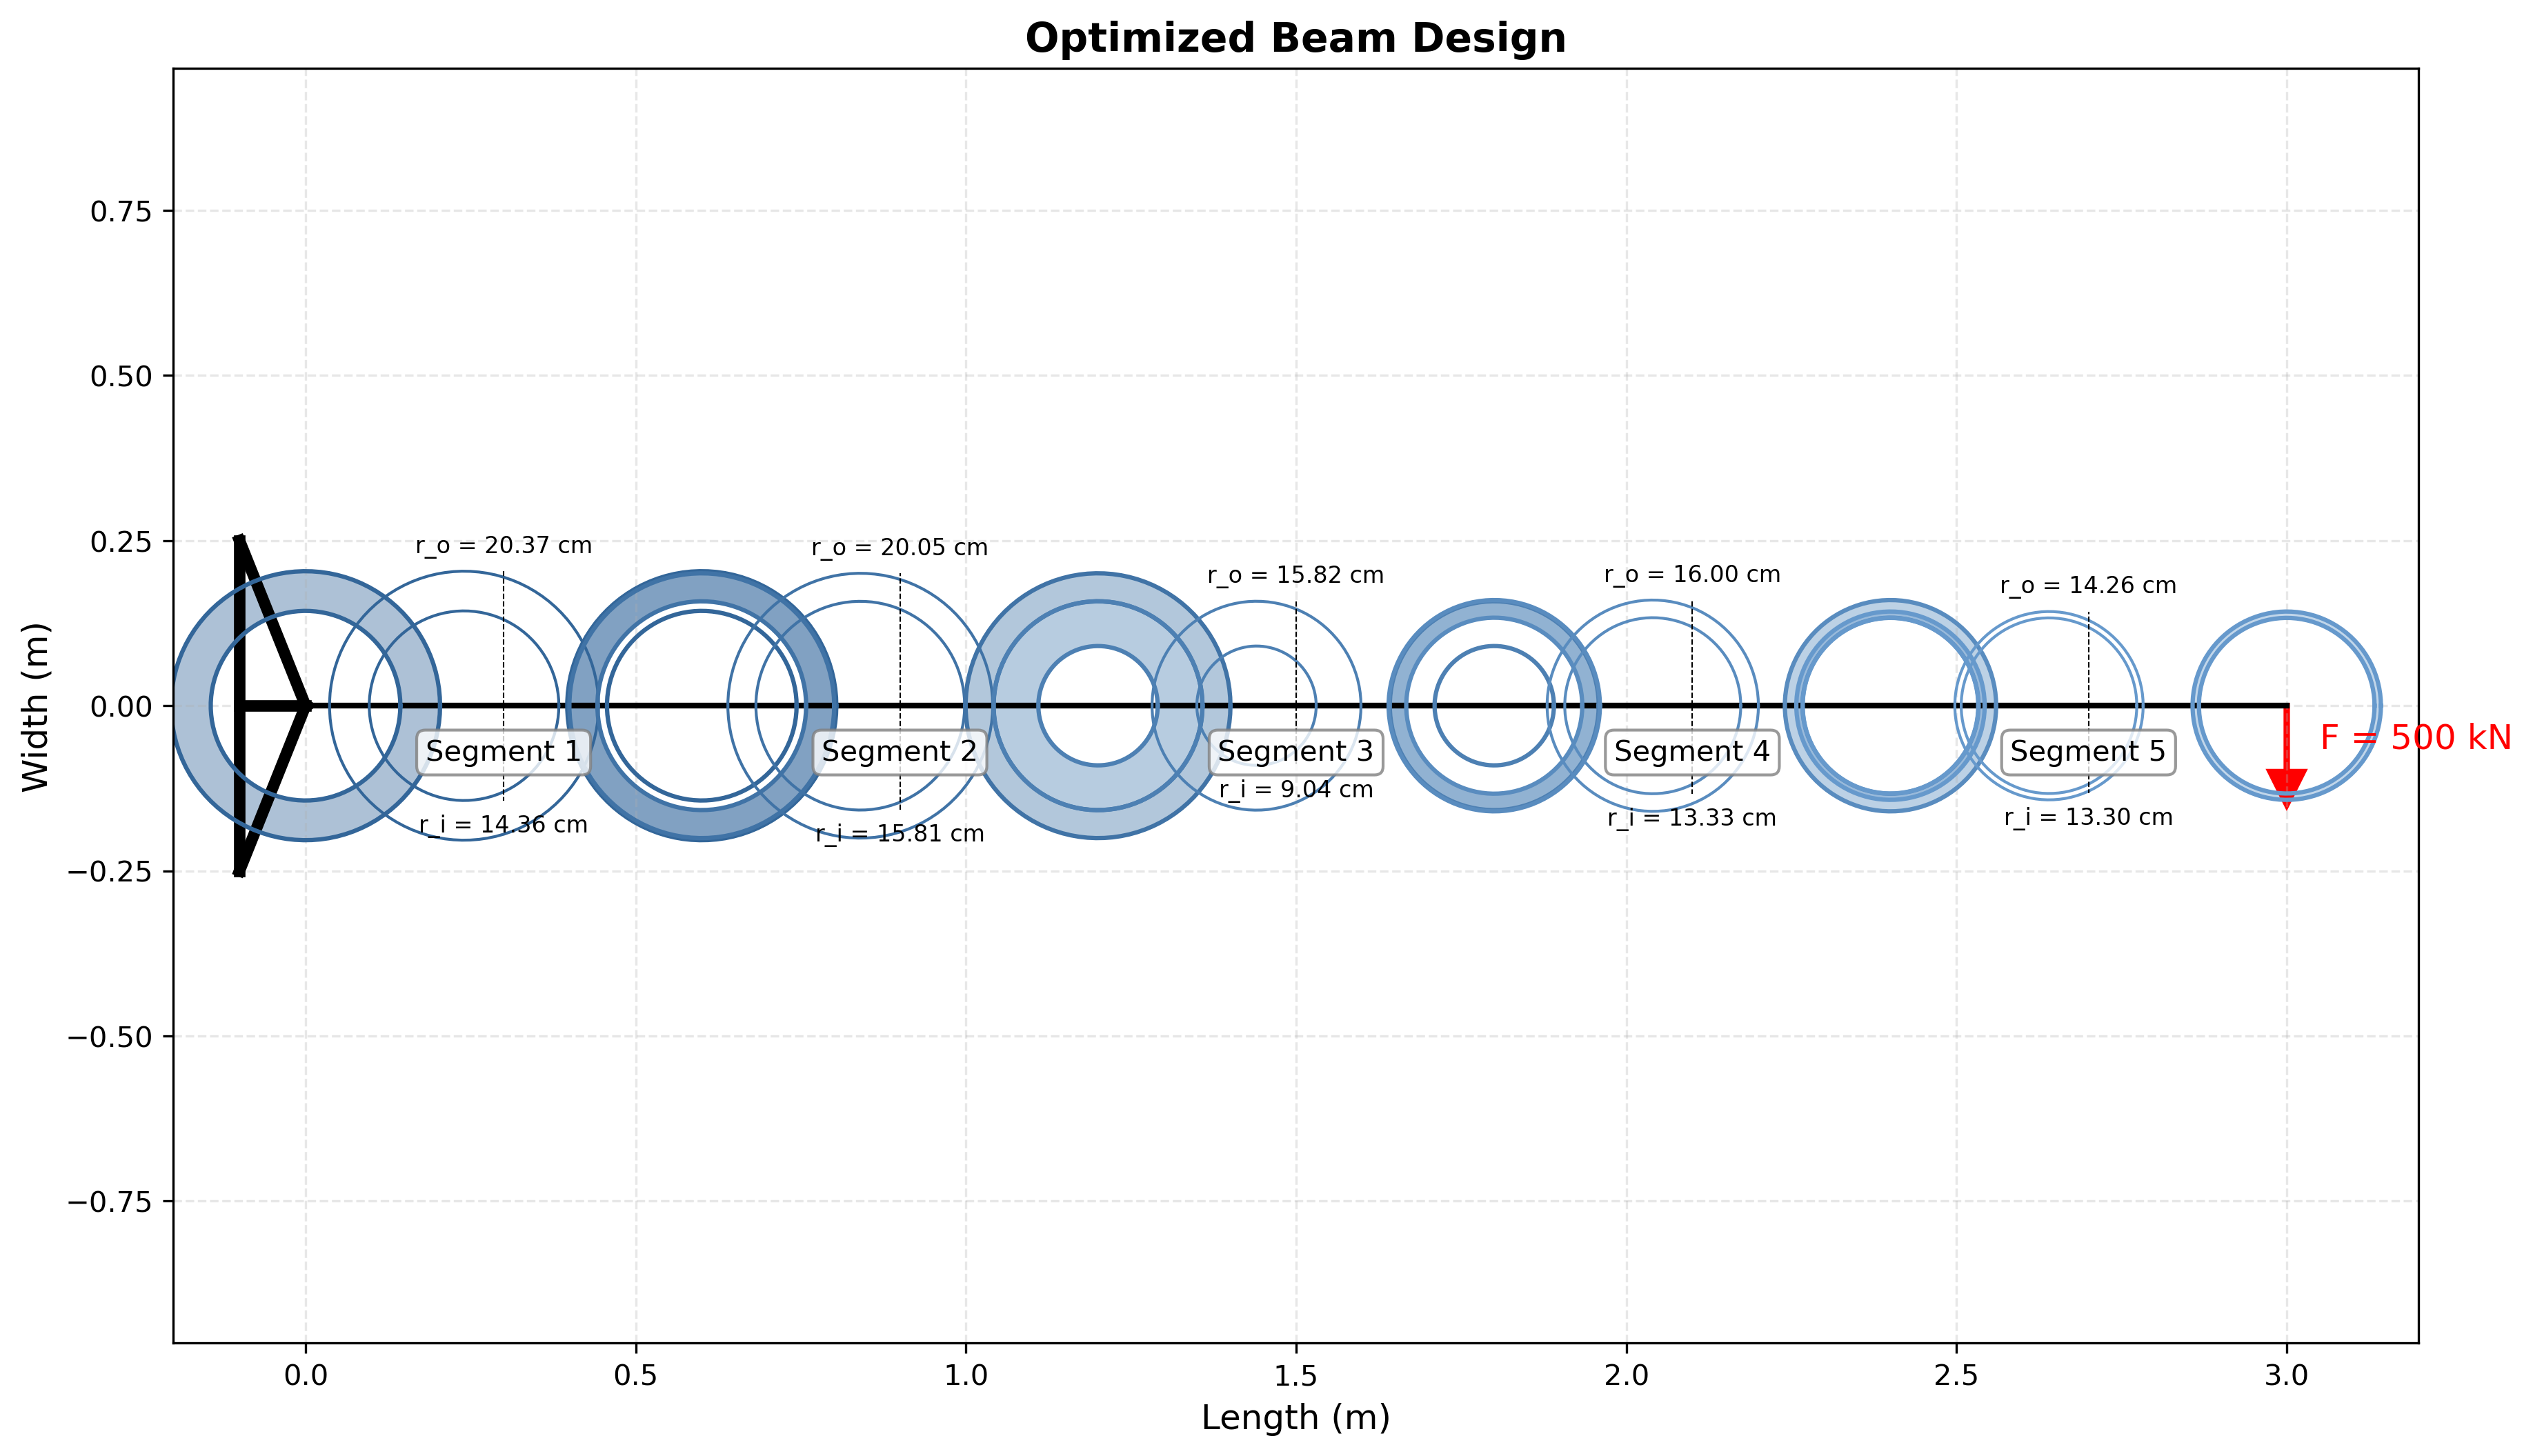
\includegraphics[width=1\textwidth]{weeks_new/imgs/optimized_beam.png}
    \caption{Optimize Edilmiş Kiriş Tasarımı}
    \label{fig:optimized_beam}
\end{figure}

\subsubsection{Deformasyon Şekli}
Yük altındaki konsol kirişin deformasyon şekli, serbest uçta maksimum 2 cm'lik bir deplasmana sahiptir. Her düğüm noktasındaki deplasman değerleri de gösterilmiştir.

\begin{figure}[H]
    \centering
    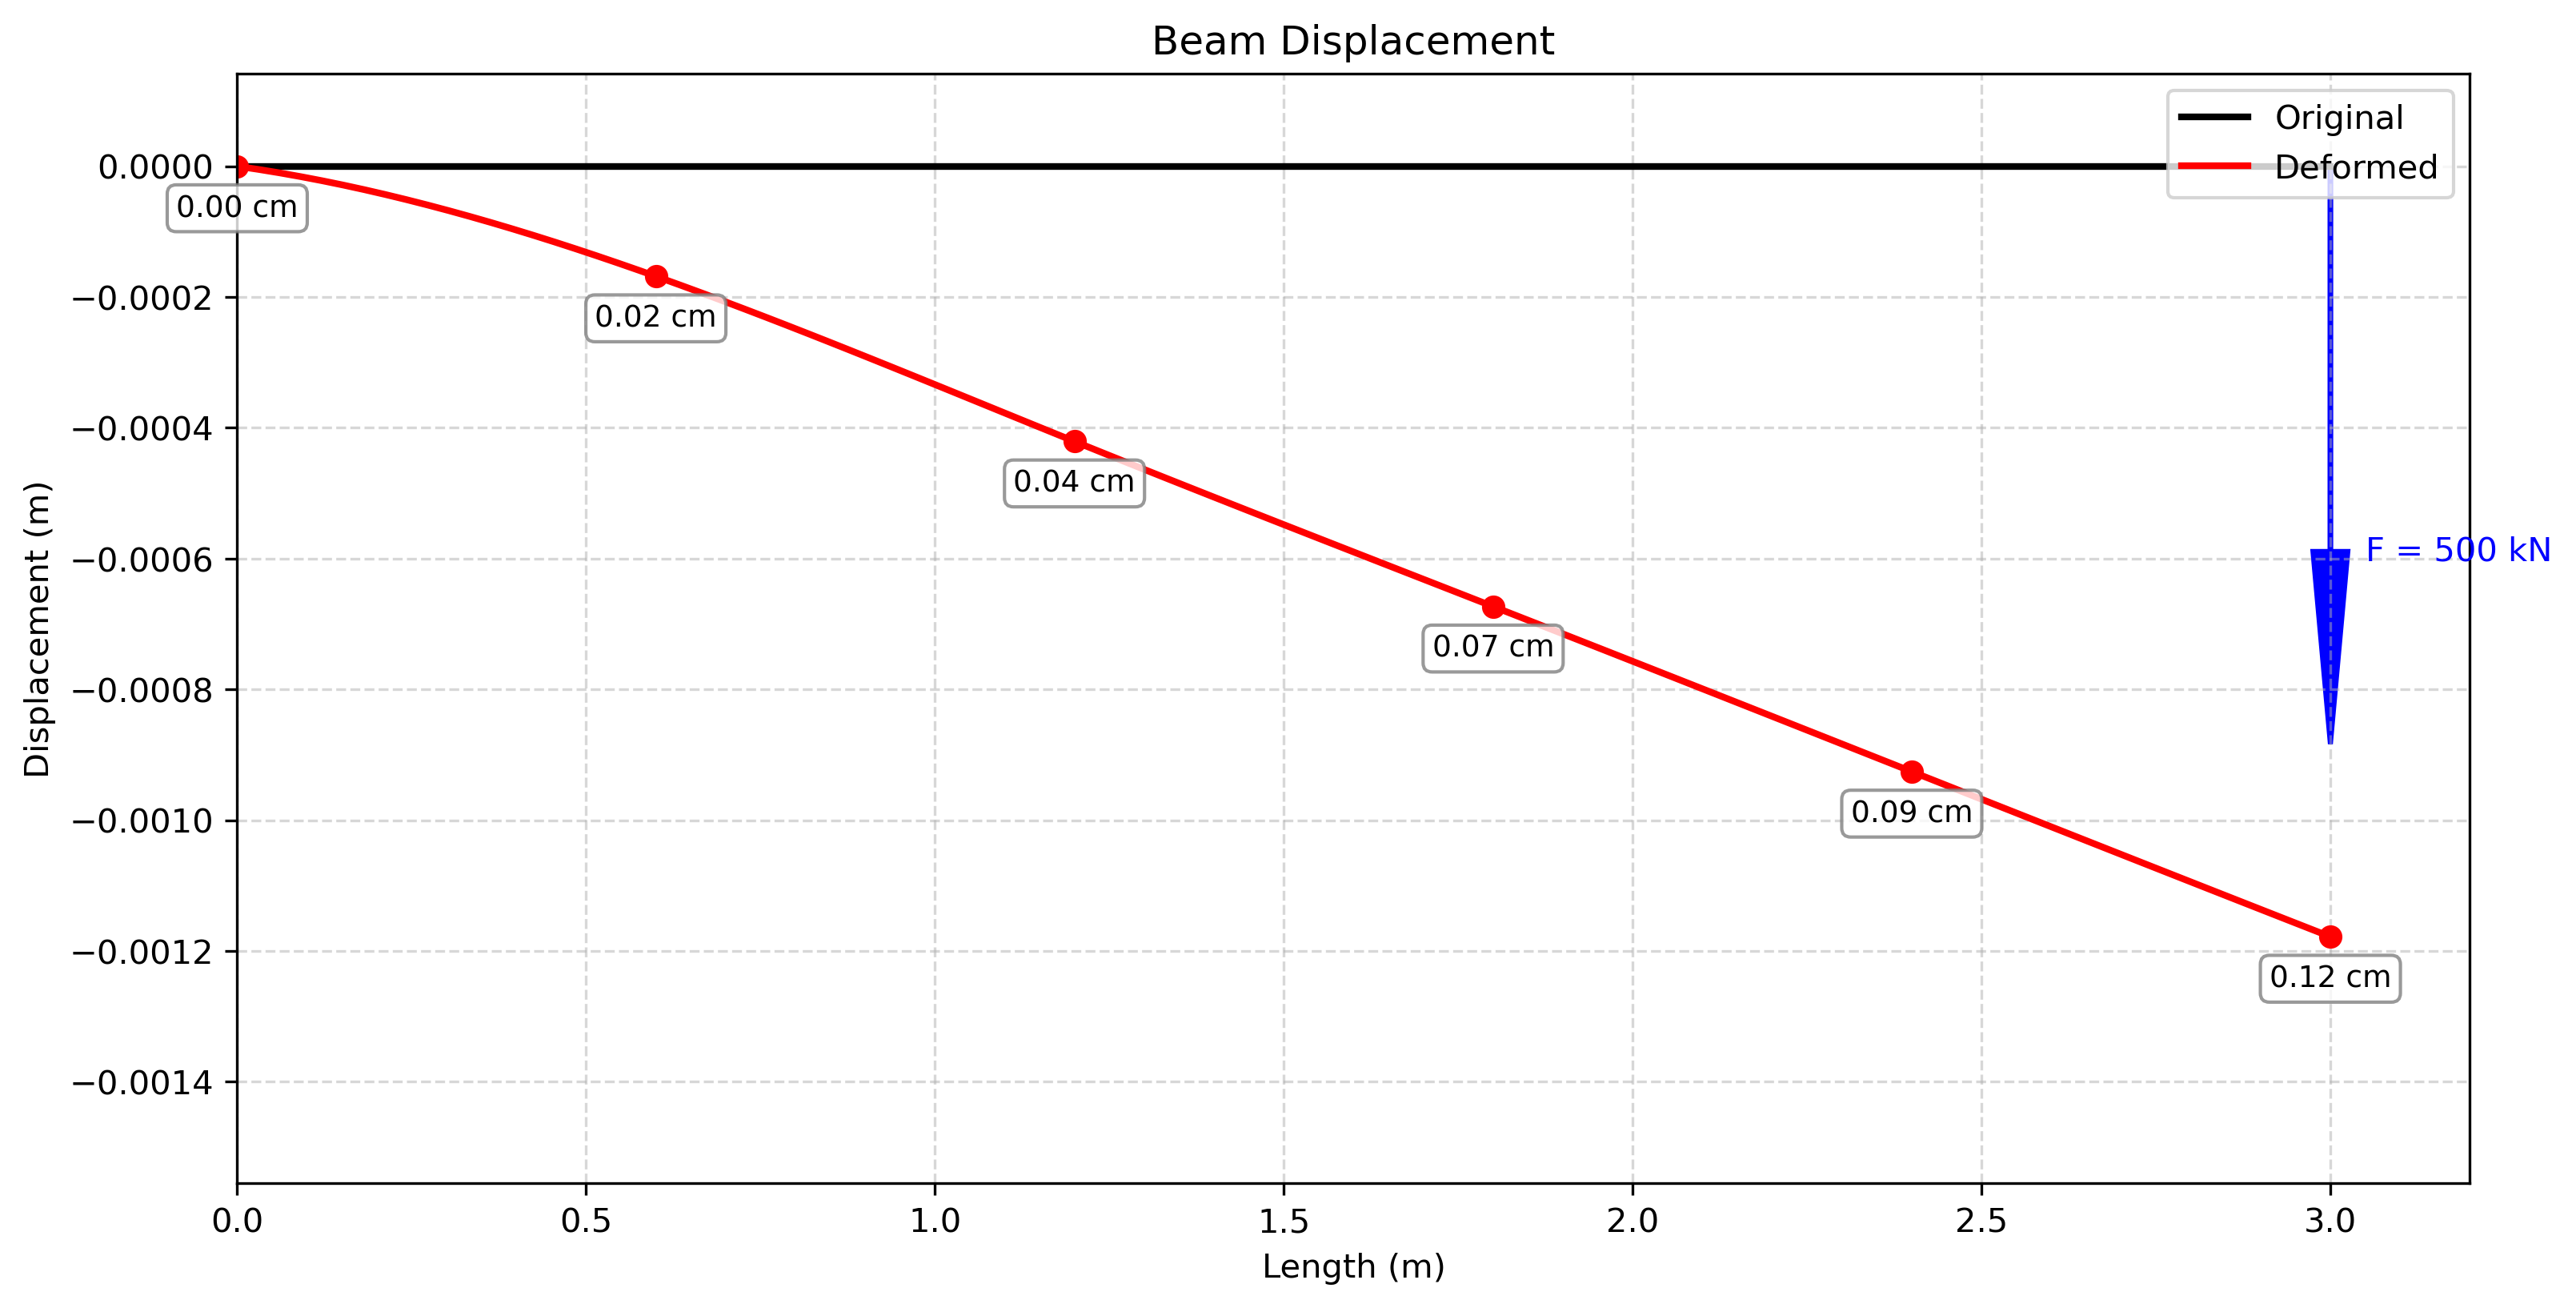
\includegraphics[width=1\textwidth]{weeks_new/imgs/deformed_beam.png}
    \caption{Deformasyon Şekli}
    \label{fig:deformed_beam}
\end{figure}

\subsubsection{Kısıtlama Kullanım Oranları}
Optimize edilmiş tasarımda her bir kısıtlamanın ne kadar kullanıldığını gösteren grafikler oluşturulmuştur:

\begin{itemize}
    \item \textbf{Deplasman Kısıtlaması}: Maksimum deplasman sınırı tamamen kullanılmıştır (\%100)
    \item \textbf{Gerilme Kısıtlaması}: Her segment için akma gerilmesinin kullanım oranı
    \item \textbf{Yarıçap Oranı}: İç yarıçapın dış yarıçapa oranı
    \item \textbf{Kaynak Yapılabilirlik}: Bitişik segmentler arasındaki kaynak koşulunun kullanım oranı
\end{itemize}

\begin{figure}[H]
    \centering
    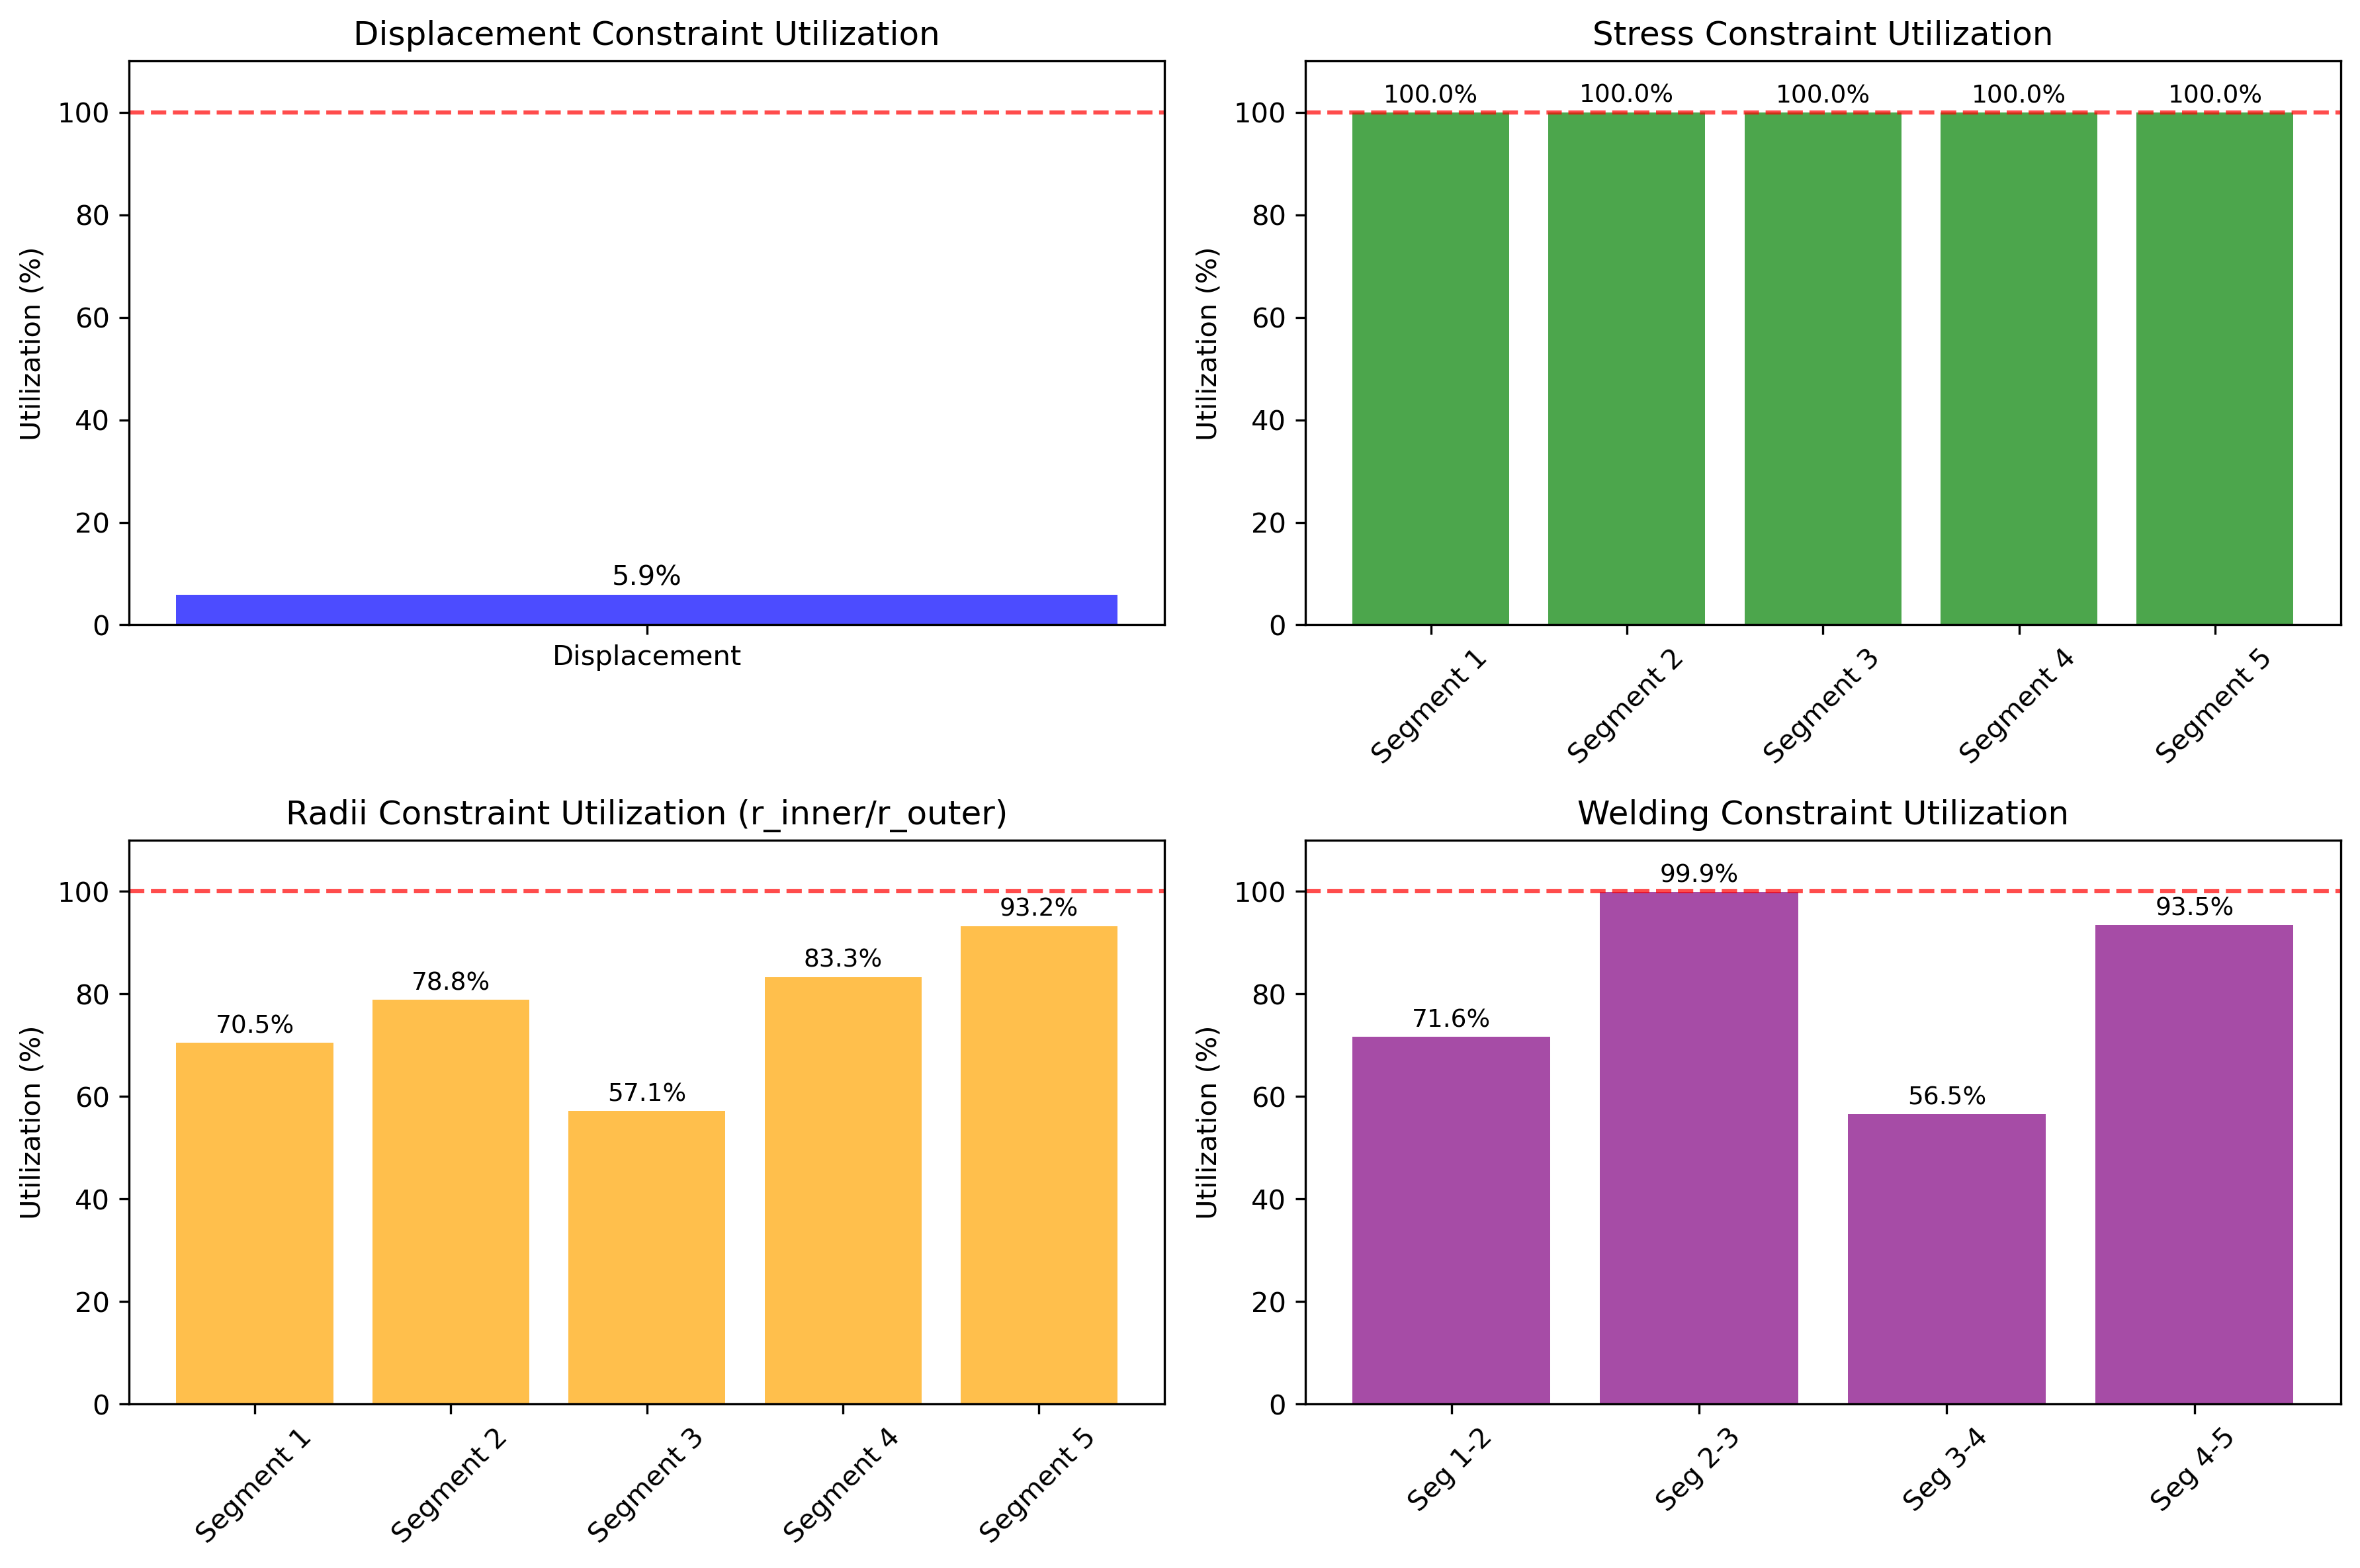
\includegraphics[width=1\textwidth]{weeks_new/imgs/constraint_utilization.png}
    \caption{Sınırlayıcı Kapasite Kullanım Oranları}
    \label{fig:constraint_utilization}
\end{figure}

Grafiklerden görüldüğü üzere, optimal tasarımda deplasman kısıtlaması aktiftir (tamamen kullanılmıştır). Bu, optimize edilmiş tasarımın ağırlık minimizasyonu açısından limite ulaştığını göstermektedir.

\subsection{Sonuç ve Değerlendirme}
Bu uygulamada, Benzetimli Tavlama optimizasyon algoritması kullanılarak, kısıtlamalar altında minimum ağırlık için bir konsol kirişin optimal tasarımı elde edilmiştir. Sonuçlar, başlangıç tasarımından \%51 daha hafif bir yapının elde edildiğini göstermektedir.

Optimize edilmiş tasarımda, özellikle gerilme kısıtlamasının tamamen kullanıldığı (aktif olduğu) gözlemlenmektedir. Bu, ağırlık minimizasyonu problemlerinde teorik olarak beklenen bir sonuçtur, çünkü tipik olarak en az bir kısıtlamanın aktif olması beklenir.

Destek noktasından serbest uca doğru kiriş geometrisinin kademeli olarak azalması da yapısal açıdan beklenen bir sonuçtur. Eğilme momenti destek noktasında maksimum olduğundan, bu bölgede daha büyük kesitler oluşmuştur.